\documentclass[11pt,a4paper]{jsarticle}
%
\usepackage{amsmath,amssymb}
\usepackage{bm}
\usepackage[dvipdfmx]{graphicx}
\usepackage[dvipdfmx]{color}
\usepackage{ascmac}
\usepackage{listings}
%
\setlength{\textwidth}{\fullwidth}
\setlength{\textheight}{40\baselineskip}
\addtolength{\textheight}{\topskip}
\setlength{\voffset}{-0.2in}
\setlength{\topmargin}{0pt}
\setlength{\headheight}{0pt}
\setlength{\headsep}{0pt}
%
\newcommand{\divergence}{\mathrm{div}\,}  %ダイバージェンス
\newcommand{\grad}{\mathrm{grad}\,}  %グラディエント
\newcommand{\rot}{\mathrm{rot}\,}  %ローテーション
%
\title{レポート課題11}
\author{05-191009 奥村真司}
\date{}
\begin{document}
\maketitle
%
%
\section*{問1}
\subsection*{考察}
以下のように探索が無限ループするため期待どおりに動かない。
$$ancestor(kobo,iwao)\ \ \ \rightarrow$$
$$ancestor(Z_1,iwao),parent(kobo,Z_1)\ \ \ \rightarrow$$
$$ancestor(Z_2,iwao),parent(Z_1,Z_2),parent(kobo,Z_1)\ \ \ \rightarrow...$$
前回の授業でやったとおり、
\begin{lstlisting}[basicstyle=\ttfamily\footnotesize, frame=single]
ancestor(X,Y) :- parent(X,Z),ancestor(Z,Y).
ancestor(X,Y) :- parent(X,Y).
\end{lstlisting}
とすればZが決まりやすく、期待通り動作する。
\section*{問2}
\subsection*{考察}
探索は以下の画像のように進む。\\
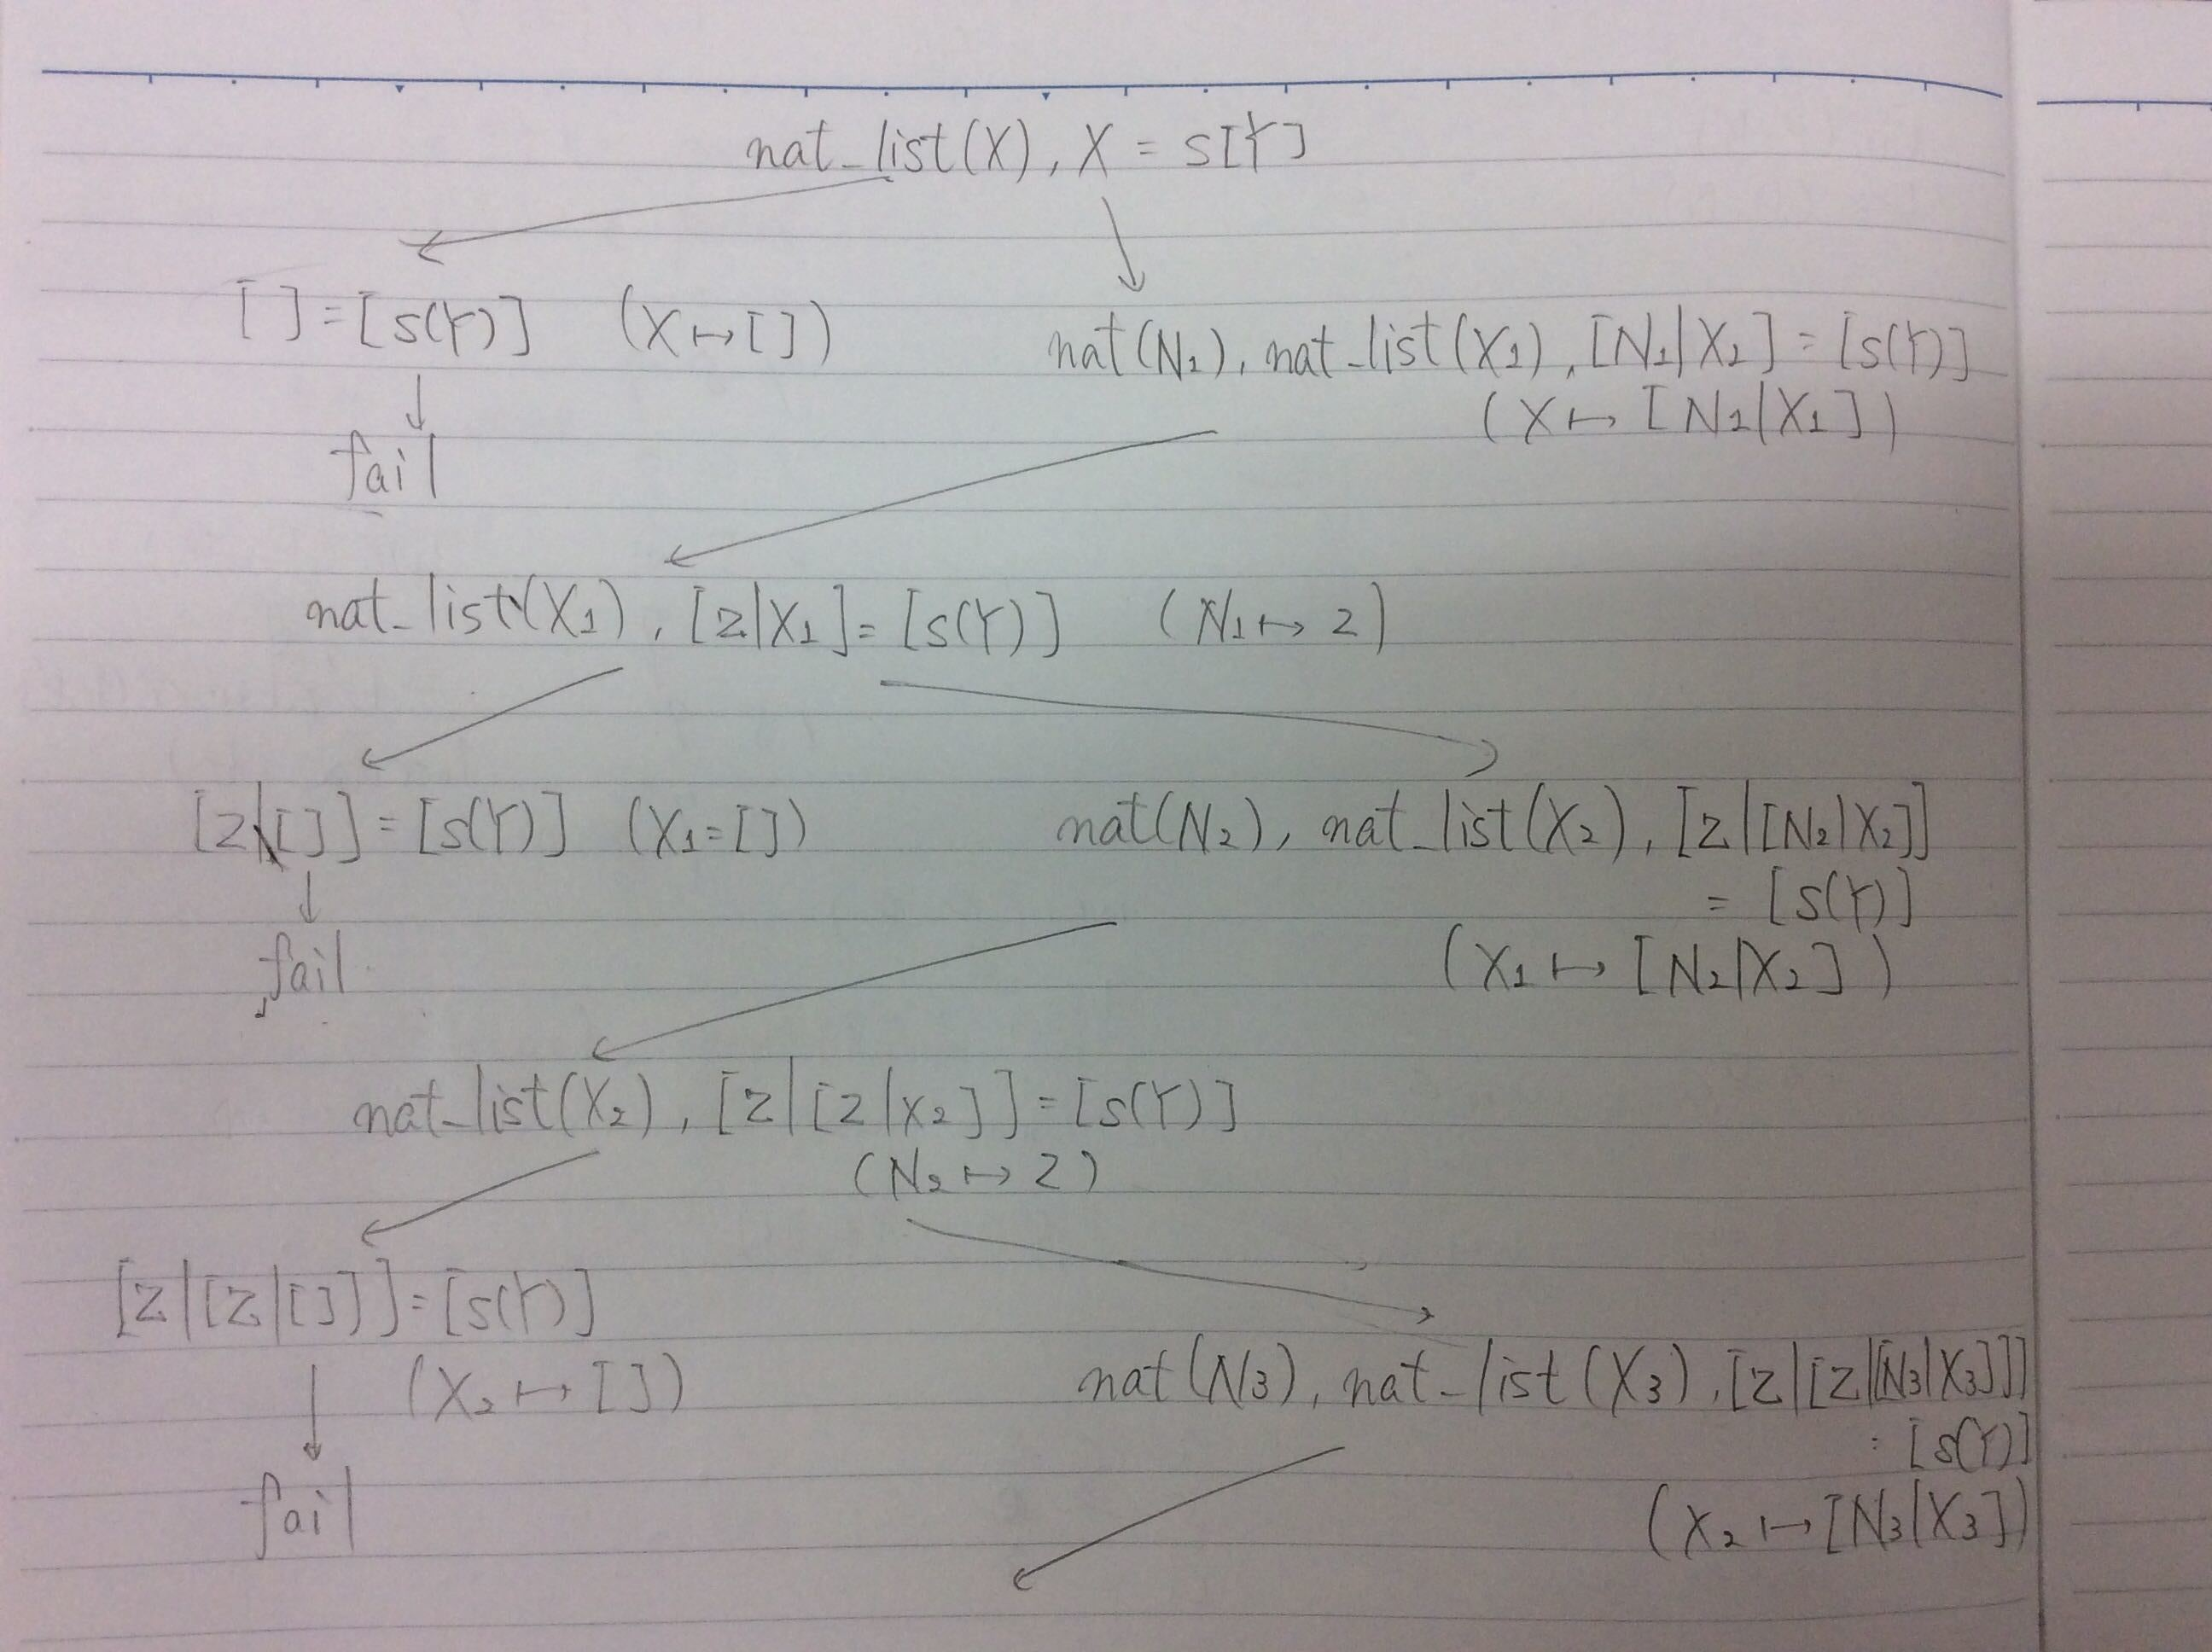
\includegraphics[width=14.5cm]{problem2.jpg}\par
図のように、$nat(N_k),nat\_list(X_k),[z|[z|..|[N_k|X_k]..]]]]=[s(Y)]$
の形の状態が現れ続け、無限に探索が終わらない。
以下のように
\begin{lstlisting}[basicstyle=\ttfamily\footnotesize, frame=single]
nat(z).
nat(s(N)) :- nat(N).
nat_list([]).
nat_list([N|X]) :- nat_list(X),nat(N).
\end{lstlisting}
として(4行目のnat,nat\_listの順序を入れ替えた)リストの要素が自然数かチェックするより先にリストの形を決めてやることで探索範囲をせばめてやると、期待通り動作するようになった。
\section*{問3}
\subsection*{動作例}
\begin{lstlisting}[basicstyle=\ttfamily\footnotesize, frame=single]
?- ['family.pl'].
true.

?- win(a,[e,e,e,e,e,e,e,e,e]).
false.

?- lose(a,[e,e,e,e,e,e,e,e,e]).
false.

?- win(a,[a,e,e,b,e,e,e,e,e]).
true .

?- win(a,[e,e,e,b,a,e,e,e,e]).
true .

?- win(a,[e,a,e,b,e,e,e,e,e]).
true .
\end{lstlisting}
\subsection*{考察}
実装にあたって定義したPredicateの説明をする。
$$end(P,B) \Leftrightarrow 盤面BでプレイヤーPがすでに勝っている(3つならべている)$$ 
$$enemy(P,Q) \Leftrightarrow Pの相手がQ$$
$$next(P,B,C) \Leftrightarrow Pの手番で盤面Bの状態から盤面Cの状態になりうる$$
$$notfull(B) \Leftrightarrow 盤面Bで空きマスがある$$
を実装した。
loseの実装の際に全称量化子が必要になるが、Prologで自然に書けるPredicateは限定量化子のついた形だと思ったので先頭に2重否定をつけ、内側の否定を全称量化子の中に入れて量化子を存在量化子に変えて実装した。すなわち、loseで
$$next(P,B,C)なる任意の局面Cについてwin(Q,C)$$
を
$$(next(P,B,C)なるある局面Cが存在してwin(Q,C)でない)でない$$
とした。これらを用いてwin,loseは
\begin{lstlisting}[basicstyle=\ttfamily\footnotesize, frame=single]
win(P,B) :- end(P,B).
win(P,B) :- enemy(P,Q),\+end(Q,B),next(P,B,C),lose(Q,C).
notwin(P,B) :- \+ win(P,B).
notlose(P,Q,B) :- next(P,B,C),notwin(Q,C).
lose(P,B) :- enemy(P,Q),end(Q,B).
lose(P,B) :- enemy(P,Q),\+end(P,B),notfull(B),\+ notlose(P,Q,B).
\end{lstlisting}
のように実装できた。
このPredicateでは探索していくので順次未決定な部分が決まっていく。なので否定はあまり深く考えずに述語論理と対応させて用いた。
動作例のはじめの2つから、先手後手ともに必勝法がないことがわかる。
また授業スライド内の各盤面状態が先手必勝であることも確認できた。
\section*{問}
\subsection*{動作例}
\begin{lstlisting}[basicstyle=\ttfamily\footnotesize, frame=single]
\end{lstlisting}
\subsection*{考察}
\end{document}
